\documentclass[12pt, twoside]{article}
\usepackage[letterpaper, margin=1in, headsep=0.5in]{geometry}
\usepackage[english]{babel}
\usepackage[utf8]{inputenc}
\usepackage{amsmath}
\usepackage{amsfonts}
\usepackage{amssymb}
\usepackage{tikz}
\usetikzlibrary{quotes, angles}
\usepackage{graphicx}
\usepackage{enumitem}
\usepackage{multicol}

\newif\ifmeta
\metatrue %print standards and topics tags

\title{Regents Geometry}
\author{Chris Huson}
\date{February 2022}

\usepackage{fancyhdr}
\pagestyle{fancy}
\fancyhf{}
\renewcommand{\headrulewidth}{0pt} % disable the underline of the header
\raggedbottom

\fancyhead[LE]{\thepage}
\fancyhead[RO]{\thepage \\ Name: \hspace{4cm} \,\\}
\fancyhead[LO]{BECA / Dr. Huson / Geometry 7 Similarity}

\begin{document}

\subsubsection*{7.7 Similar triangles \hfill CCSS.HSG.SRT.B.5}
\begin{enumerate}
\item Do Now: Triangle $ABC$ is dilated with a factor of $\frac{3}{2}$ centered at $A$, yielding $\triangle ADE$, as shown. Given $AB=10$, $BC=12$, and $AC=14$. \\[0.25cm] Find $AD$, $AE$, and $DE$.
  \begin{flushright}
    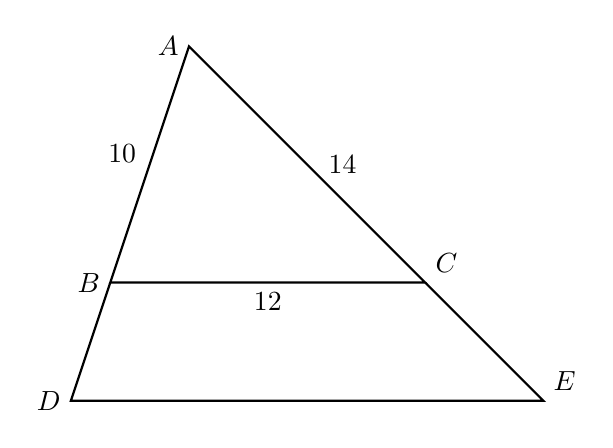
\begin{tikzpicture}[scale=0.5]
      \draw [thick]
      (0,0)node[left]{$B$}--
      (8,0)node[above right]{$C$}--
      (2,6)node[left]{$A$}--cycle;
      \draw [thick]
      (0,0)--
      (-1,-3)node[left]{$D$}--
      (11,-3)node[above right]{$E$}--(8,0);
      \node at (4,0)[below]{$12$};
      \node at (5.3, 3)[right]{$14$};
      \node at (0.3, 2.8)[above]{$10$};
    \end{tikzpicture}
    \end{flushright} \vspace{1cm}

\item Given $\triangle ABP \sim \triangle JKP$. $AB=8$, $AP=7.0$, $KP=7.875$, $JK=14.0$, $m\angle A=20^\circ$, $m\angle JPK = 110^\circ$. Mark the given values on the diagram, find the scale factor, and solve the triangles (all angles and lengths).
  \begin{center}
    \begin{tikzpicture}[scale=1.8]
        \draw [thick]
          (0.25,-1)node[right]{$B$}--
          (-0.5,2)node[left]{$K$}--
          (4,0)node[right]{$J$}--
          (0,0)node[above right]{$P$}--
          (-2,0)node[left]{$A$}--cycle;
      \end{tikzpicture}
  \end{center}

\newpage
\item Triangle $ADE$ and its midline $\overline{BC}$ are drawn, with $B$ the midpoint of $\overline{AD}$ and $C$ the midpoint of $\overline{AE}$. The two medians $\overline{BE}$ and $\overline{CD}$ are drawn, as shown, intersecting in point $F$, the centroid.
\begin{multicols}{2}
  $\triangle FCB \sim \triangle FDE$ with scale factor $k=2$.\\[0.25cm]
  Given $BC=7$, find $DE$. \\[0.25cm] Given $BF=4$, find $FE$. \vspace{1cm}
  \begin{center}
      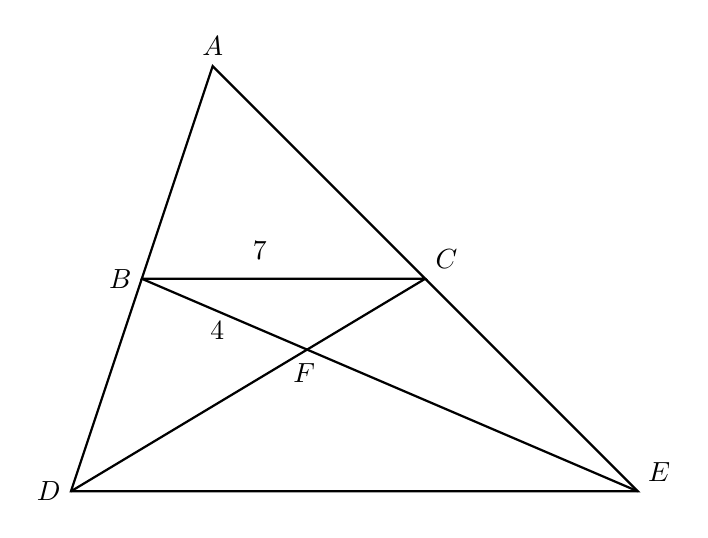
\begin{tikzpicture}[scale=0.6]
        \draw [thick]
        (0.5,1.5)node[left]{$B$}--
        (6.5,1.5)node[above right]{$C$}--
        (2,6)node[above]{$A$}--cycle;
        \draw [thick]
        (0.5,1.5)--
        (-1,-3)node[left]{$D$}--
        (11,-3)node[above right]{$E$}--(6.5,1.5);
        \draw [thick] (0.5,1.5)--(11,-3);
        \draw [thick] (6.5,1.5)--(-1,-3);
        \node at (3,2.5)[below]{$7$};
        \node at (3.5, -0.5)[right]{$F$};
        \node at (2.1, 0)[above]{$4$};
        %\node at (-0.7, -1)[above]{$5$};
      \end{tikzpicture}
    \end{center}
\end{multicols} \vspace{2cm}

\item Regents problem: In triangle $ABC$, points $D$ and $E$ are on sides of $\overline{AB}$ and $\overline{BC}$, respectively, such that $\overline{DE} \parallel \overline{AC}$, and $AD:DB = 3:5$.
\begin{center}
  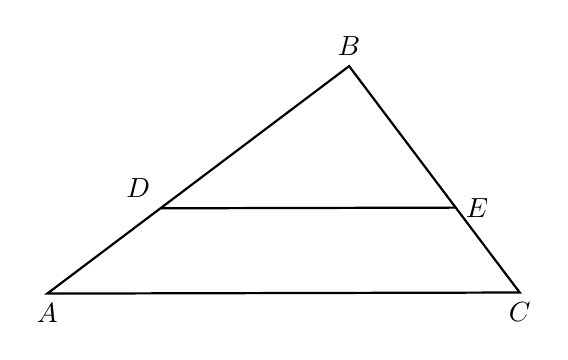
\begin{tikzpicture}[scale=0.6, rotate=-13]
    \draw [thick]
    (0,0)node[above]{$B$}--
    (-130:8)node[below]{$A$}--
    (-40:6)node[below]{$C$}--cycle;
    \draw [thick]
    (-130:5)node[above left]{$D$}--
    (-40:3.75)node[right]{$E$};
  \end{tikzpicture}
\end{center}
If $DB=6.3$ and $AC=9.4$, what is the length of $\overline{DE}$, to the \emph{nearest tenth}?

\newpage
\item A dilation maps $\triangle ABC \rightarrow \triangle ADE$. Given $AB=9$, $AC=11.1$, $BC=6$, $DE=14$. 
\begin{multicols}{2}
  Find the scale factor and side lengths:\\[0.5cm]
  $k=$\\[1cm]
  $AD=$\\[1cm]
  $AE=$\\[1cm]
  $BD=$\\
  \begin{flushright}
    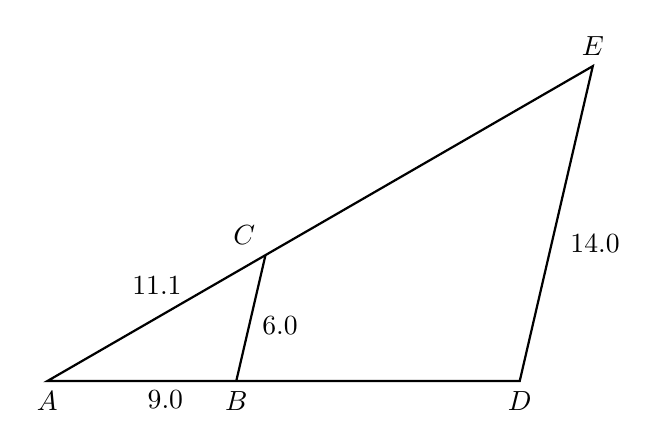
\begin{tikzpicture}[scale=1.]
      \draw [thick]
      (0,0)node[below]{$A$}--
      (0:6)node[below]{$D$}--
      (30:8)node[above]{$E$}--cycle;
      \draw [thick]
      (0:2.4)node[below]{$B$}--
      (30:3.2)node[above left]{$C$};
      \node at (0:1.5)[below]{$9.0$};
      \node at (15:2.7)[right]{$6.0$};
      \node at (15:6.75)[right]{$14.0$};
      \node at (35:1.7)[above]{$11.1$};
    \end{tikzpicture}
  \end{flushright}
\end{multicols}\vspace{0.25cm}

\item Steven and Marie live close to school and Tio's bodega, but also like to go to Grandma's house and the baseball field, which are further away. A sketch of the locations is shown below, essentially two triangles with a scale factor $k=2$ centered at home.\\[0.25cm]
From home it's 4 blocks to school and 3 to the bodega. From Grandma's to the baseball field is 10 blocks. There are twenty blocks to a mile.
\begin{enumerate}
  \item Steven stops at the bodega on his way to school. How far does he walk, in terms of both blocks and miles?
\begin{flushright}
  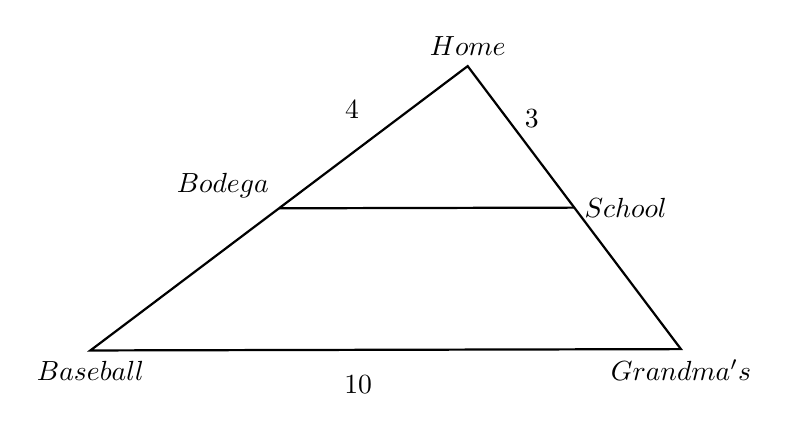
\begin{tikzpicture}[scale=0.6, rotate=-13]
    \draw [thick]
    (0,0)node[above]{$Home$}--
    (-130:10)node[below]{$Baseball$}--
    (-40:7.5)node[below]{$Grandma's$}--cycle;
    \draw [thick]
    (-130:5)node[above left]{$Bodega$}--
    (-40:3.75)node[right]{$School$};
    \node at (-155:2.5)[below]{$4$};
    \node at (-35:1.5)[right]{$3$};
    \node at (-95:7.5)[above]{$10$};
  \end{tikzpicture}
\end{flushright} 
  \item Marie goes to play baseball from school. Which way is shorter, passing by the bodega or the route by Grandma's? By how many blocks is it shorter? Justify your answer.
\end{enumerate}

\newpage
\item Given $\triangle ABP \sim \triangle JKP$. $AB=7$, $AP=6.3$, $KP=8.8$, $JK=16.0$, $m\angle A=25^\circ$, $m\angle JPK = 105^\circ$. Solve the triangles (all angles and lengths).
\begin{flushright}
  \begin{tikzpicture}[scale=1.6]
      \draw [thick]
        (0.25,-1)node[right]{$B$}--
        (-0.5,2)node[left]{$K$}--
        (4,0)node[right]{$J$}--
        (0,0)node[above right]{$P$}--
        (-2,0)node[left]{$A$}--cycle;
    \end{tikzpicture}
\end{flushright} \vspace{2cm}
  
\item Triangle $ADE$ is drawn with $\overline{BC} \parallel \overline{DE}$, as shown. Given $AB=5$, $BC=8$, $AC=8$, and $BD=5$. $m\angle A = 72^\circ$. \\[0.25cm] Find $CE$, $AE$, and $DE$. Find and mark all of the angle measures of the triangle.\vspace{1cm}
\begin{flushright}
  \begin{tikzpicture}[scale=0.65]
    \draw [thick]
    (0.5,1.5)node[left]{$B$}--
    (6.5,1.5)node[above right]{$C$}--
    (2,6)node[above]{$A$}--cycle;
    \draw [thick]
    (0.5,1.5)--
    (-1,-3)node[left]{$D$}--
    (11,-3)node[above right]{$E$}--(6.5,1.5);
    \node at (3,1.5)[below]{$8$};
    \node at (4.5, 4)[right]{$8$};
    \node at (0.6, 3.3)[above]{$5$};
    \node at (-0.7, -1)[above]{$5$};
  \end{tikzpicture}
\end{flushright}

\end{enumerate}
\end{document}
